%%%%%%%%%%%%%%%%%%%%%%%%%%%%%%%%%%%%%%%%%%%%%%%%%%%%%%%%%%%%%%%%%%%%% 
%% This is a (brief) model paper using the achemso class 
%% The document class accepts keyval options, which should include 
%% the target journal and optionally the manuscript type. 
%%%%%%%%%%%%%%%%%%%%%%%%%%%%%%%%%%%%%%%%%%%%%%%%%%%%%%%%%%%%%%%%%%%%% 
\documentclass[journal=jpcbfk,manuscript=article]{achemso} 
 
%%%%%%%%%%%%%%%%%%%%%%%%%%%%%%%%%%%%%%%%%%%%%%%%%%%%%%%%%%%%%%%%%%%%% 
%% Place any additional packages needed here.  Only include packages 
%% which are essential, to avoid problems later. Do NOT use any 
%% packages which require e-TeX (for example etoolbox): the e-TeX 
%% extensions are not currently available on the ACS conversion 
%% servers. 
%%%%%%%%%%%%%%%%%%%%%%%%%%%%%%%%%%%%%%%%%%%%%%%%%%%%%%%%%%%%%%%%%%%%% 
 
\usepackage{rotating}  
\usepackage{times} 
\usepackage{graphicx} 
\usepackage{setspace} 
\usepackage{amsmath} 
\usepackage{epstopdf} 
\usepackage{csquotes} 
\usepackage{mhchem} 
\usepackage{chemfig} 
\usepackage[obeyFinal]{easy-todo}
 
%\usepackage{markdown}  
 
 
%%%%%%%%%%%%%%%%%%%%%%%%%%%%%%%%%%%%%%%%%%%%%%%%%%%%%%%%%%%%%%%%%%%%% 
%% If issues arise when submitting your manuscript, you may want to 
%% un-comment the next line.  This provides information on the 
%% version of every file you have used. 
%%%%%%%%%%%%%%%%%%%%%%%%%%%%%%%%%%%%%%%%%%%%%%%%%%%%%%%%%%%%%%%%%%%%% 
%%\listfiles 
 
%%%%%%%%%%%%%%%%%%%%%%%%%%%%%%%%%%%%%%%%%%%%%%%%%%%%%%%%%%%%%%%%%%%%% 
%% Place any additional macros here.  Please use \newcommand* where 
%% possible, and avoid layout-changing macros (which are not used 
%% when typesetting). 
%%%%%%%%%%%%%%%%%%%%%%%%%%%%%%%%%%%%%%%%%%%%%%%%%%%%%%%%%%%%%%%%%%%%% 
\newcommand*\mycommand[1]{\texttt{\emph{#1}}} 
\newlength{\figwidth}
\setlength{\figwidth}{8 cm}

 
%%%%%%%%%%%%%%%%%%%%%%%%%%%%%%%%%%%%%%%%%%%%%%%%%%%%%%%%%%%%%%%%%%%%% 
%% Meta-data block 
%% --------------- 
%% Each author should be given as a separate \author command. 
%% 
%% Corresponding authors should have an e-mail given after the author 
%% name as an \email command. Phone and fax numbers can be given 
%% using \phone and \fax, respectively; this information is optional. 
%% 
%% The affiliation of authors is given after the authors; each 
%% \affiliation command applies to all preceding authors not already 
%% assigned an affiliation. 
%% 
%% The affiliation takes an option argument for the short name.  This 
%% will typically be something like "University of Somewhere". 
%% 
%% The \altaffiliation macro should be used for new address, etc. 
%% On the other hand, \alsoaffiliation is used on a per author basis 
%% when authors are associated with multiple institutions. 
%%%%%%%%%%%%%%%%%%%%%%%%%%%%%%%%%%%%%%%%%%%%%%%%%%%%%%%%%%%%%%%%%%%%% 
 
\author{Josef Melcr} 
\email{melcr@uochb.cas.cz} 
%%\homepage[]{https://jmelcr.github.io/}
\affiliation{Institute of Organic Chemistry and Biochemistry, 
Academy of Sciences of the Czech Republic,  
Prague 6, Czech Republic} 
\author{Pavel Jungwirth} 
%%\homepage[]{http://jungwirth.uochb.cas.cz/}
\affiliation{Institute of Organic Chemistry and Biochemistry, 
Academy of Sciences of the Czech Republic,  
Prague 6, Czech Republic} 
\alsoaffiliation{Department of Physics, Tampere University of Technology, P.O. Box 692, FI-33101 
Tampere, Finland} 
 
\author{O. H. Samuli Ollila} 
\email{samuli.ollila@helsinki.fi} 
%%\homepage[]{Your web page} 
\affiliation{Institute of Organic Chemistry and Biochemistry, 
Academy of Sciences of the Czech Republic,  
Prague 6, Czech Republic} 
\alsoaffiliation{Institute of Biotechnology, University of Helsinki} 
 
 
%\author{Andrew N. Other} 
%\altaffiliation{A shared footnote} 
%\author{Fred T. Secondauthor} 
%\altaffiliation{Current address: Some other place, Othert\"own, 
%Germany} 
%\author{I. Ken Groupleader} 
%\altaffiliation{A shared footnote} 
%\email{i.k.groupleader@unknown.uu} 
%\phone{+123 (0)123 4445556} 
%\fax{+123 (0)123 4445557} 
%\affiliation[Unknown University] 
%{Department of Chemistry, Unknown University, Unknown Town} 
%\alsoaffiliation[Second University] 
%{Department of Chemistry, Second University, Nearby Town} 
%\author{Susanne K. Laborator} 
%\email{s.k.laborator@bigpharma.co} 
%\affiliation[BigPharma] 
%{Lead Discovery, BigPharma, Big Town, USA} 
%\author{Kay T. Finally} 
%\affiliation[Unknown University] 
%{Department of Chemistry, Unknown University, Unknown Town} 
%\alsoaffiliation[Second University] 
%{Department of Chemistry, Second University, Nearby Town} 
 
%%%%%%%%%%%%%%%%%%%%%%%%%%%%%%%%%%%%%%%%%%%%%%%%%%%%%%%%%%%%%%%%%%%%% 
%% The document title should be given as usual. Some journals require 
%% a running title from the author: this should be supplied as an 
%% optional argument to \title. 
%%%%%%%%%%%%%%%%%%%%%%%%%%%%%%%%%%%%%%%%%%%%%%%%%%%%%%%%%%%%%%%%%%%%% 
\title[] 
  {Accurate interactions of cations with 
   neutral and negatively charged membranes 
   via combination of experiments and molecular simulation}

%%%%%%%%%%%%%%%%%%%%%%%%%%%%%%%%%%%%%%%%%%%%%%%%%%%%%%%%%%%%%%%%%%%%% 
%% Some journals require a list of abbreviations or keywords to be 
%% supplied. These should be set up here, and will be printed after 
%% the title and author information, if needed. 
%%%%%%%%%%%%%%%%%%%%%%%%%%%%%%%%%%%%%%%%%%%%%%%%%%%%%%%%%%%%%%%%%%%%% 
\abbreviations{IR,NMR,UV,MD,ECC,PC,PS,POPS,POPS} 
\keywords{MD simulation, molecular modeling, 
          polarizability, polarization,
          phospholipids, phosphatidylserine} 

%%%%%%%%%%%%%%%%%%%%%%%%%%%%%%%%%%%%%%%%%%%%%%%%%%%%%%%%%%%%%%%%%%%%% 
%% The manuscript does not need to include \maketitle, which is 
%% executed automatically. 
%%%%%%%%%%%%%%%%%%%%%%%%%%%%%%%%%%%%%%%%%%%%%%%%%%%%%%%%%%%%%%%%%%%%% 
\begin{document} 
 
%%%%%%%%%%%%%%%%%%%%%%%%%%%%%%%%%%%%%%%%%%%%%%%%%%%%%%%%%%%%%%%%%%%%% 
%% The "tocentry" environment can be used to create an entry for the 
%% graphical table of contents. It is given here as some journals 
%% require that it is printed as part of the abstract page. It will 
%% be automatically moved as appropriate. 
%%%%%%%%%%%%%%%%%%%%%%%%%%%%%%%%%%%%%%%%%%%%%%%%%%%%%%%%%%%%%%%%%%%%% 
\begin{tocentry} 
 
Some journals require a graphical entry for the Table of Contents. 
This should be laid out ``print ready'' so that the sizing of the 
text is correct. 
 
Inside the \texttt{tocentry} environment, the font used is Helvetica 
8\,pt, as required by \emph{Journal of the American Chemical 
Society}. 
 
The surrounding frame is 9\,cm by 3.5\,cm, which is the maximum 
permitted for  \emph{Journal of the American Chemical Society} 
graphical table of content entries. The box will not resize if the 
content is too big: instead it will overflow the edge of the box. 
 
This box and the associated title will always be printed on a 
separate page at the end of the document. 
 
\end{tocentry} 
 
%%%%%%%%%%%%%%%%%%%%%%%%%%%%%%%%%%%%%%%%%%%%%%%%%%%%%%%%%%%%%%%%%%%%% 
%% The abstract environment will automatically gobble the contents 
%% if an abstract is not used by the target journal. 
%%%%%%%%%%%%%%%%%%%%%%%%%%%%%%%%%%%%%%%%%%%%%%%%%%%%%%%%%%%%%%%%%%%%% 
 
 
 
\begin{abstract} 
Binding affinities and stoichiometries of sodium and calcium ions to phospholipid bilayers are of paramount significance in the properties and functionality of cellular membranes. Current estimates of binding affinities and stoichiometries of cations are, however, controversial due to limitations in the available experimental and theoretical methods. Experimentally one can assess these parameters by titrating several membrane properties as a function of the ion concentration. However, the interpretation of the experiments relies on theoretical models, as direct molecular information is not available. 
Classical molecular dynamics (MD) simulations provide details of the ion binding process with atomistic resolution, therefore offering all the necessary information to interpret experimental data without the need to resort to over-simplified models. However, the accuracy of the currently available lipid models when interacting with ions is not sufficient for such interpretation \cite{catte16}. Recently, we have improved the binding details of sodium and calcium ions to the 1-Palmitoyl-2-oleoyl-phosphatidylcholine (POPC) bilayer by implicitly including electronic polarization as a mean field correction, known as the electronic continuum correction (ECC). Our improved ECC-POPC model reproduces not only the experimentally measured structural parameters for the ion-free membrane, but also improves significantly the response of lipid head group to a bound positive charge, and the binding affinities of sodium and calcium ions. \cite{melcr18}
We are now extending our work to other lipid membranes composed of larger varieties of different biologically relevant lipids. In particular, we focus our attention on membranes with phosphatidylethanolamine (PE) and negatively charged phosphatidylserine (PS). We compare available NMR and x-ray experiments with MD simulations to obtain atomistic-resolution picture of the interactions between cations and phospholipid membranes. Our preliminary results indicate that electronic polarization is a non-negligable interaction, which dramatically improves the description of cation binding to the membranes. 
\end{abstract} 
 
 
%\begin{abstract} 
%  This is an example document for the \textsf{achemso} document 
%  class, intended for submissions to the American Chemical Society 
%  for publication. The class is based on the standard \LaTeXe\ 
%  \textsf{report} file, and does not seek to reproduce the appearance 
%  of a published paper. 
 
%  This is an abstract for the \textsf{achemso} document class 
%  demonstration document.  An abstract is only allowed for certain 
%  manuscript types.  The selection of \texttt{journal} and 
%  \texttt{manuscript} will determine if an abstract is valid.  If 
%  not, the class will issue an appropriate error. 
%\end{abstract} 
 
%%%%%%%%%%%%%%%%%%%%%%%%%%%%%%%%%%%%%%%%%%%%%%%%%%%%%%%%%%%%%%%%%%%%% 
%% Start the main part of the manuscript here. 
%%%%%%%%%%%%%%%%%%%%%%%%%%%%%%%%%%%%%%%%%%%%%%%%%%%%%%%%%%%%%%%%%%%%% 
 
 
 
\section{Introduction} 
 
\section{Methods} 
 
\subsection{Electronic continuum correction for lipid bilayers}\label{section:ecc} 
This section may not be required, we may just cite ECC-POPS 
and put a short paragraph describing what we did on POPS. 

Compared to ECC-POPC model \cite{melcr18}, 
which used used a scaling factor $f_q = 0.8$ for all charges but lipid tails,
this model, ECC-POPS, has to adopt a scaling factor $f_q = 0.75$ 
as it has non-zero total charge in line with ECC theory. \cite{leontyev09}
Hence, electronic continuum correction of POPS 
has the same characteristics as for cations and anions, 
denoted as ECC-ions \cite{martinek17, Pluharova2014, kohagen14, kohagen16}. 
 
 
 
\subsection{Electrometer concept} \label{section:electrometer} 
This section may not be required, 
we may just cite ECC-POPS and NMRlipids projects papers (and ongoing works)
 
 
 
\subsection{Validation of lipid bilayer structure against NMR and scattering experiments} 
\emph{This section probably has to stay. Following text to be modified. Taken from Ref.~\citenum{melcr18}}

The structures of lipid bilayers in simulations without ions were validated against NMR by calculating the order parameters for the C-H bonds and against \mbox{X-ray} scattering experiments by evaluating the scattering form factors. 
NMR order parameters validate the structures sampled by the individual lipid molecules with atomic resolution. 
The simulated order parameters were calculated for all C-H bonds in lipid molecules from Eq. \ref{OP}.
Scattering form factors validate the dimensions of the lipid bilayer (i.e., the bilayer thickness and area per molecule). Form factors were calculated using a relation 
 
\begin{equation} 
  F(q) = \int _{-D/2} ^{D/2} \left ( \rho_{el}(z) - \rho_{el}^s \right ) \cos (zq_z) \mathrm{d}z, 
  %F(q) = \int _{-D/2} ^{D/2} \left ( \sum _\alpha f_\alpha (q_z) n_\alpha (z) - \rho _s \right ) \exp (izq_z) \mathrm{d}z, 
\end{equation} 
 
\noindent where $\rho_{el} (z)$ is the total electron density, $\rho_{el}^s$ is the electron density of the solvent far in the aqueous bulk, and $z$ is the distance from the membrane center along its normal with $D/2$ being half of the unit cell size.   

 
 
 
 
\subsection{Simulation details} 

General simulation setup.
 
\subsubsection{Simulations of POPS:POPS bilayers with aqueous ions} 

Any specifics for simulations with cations.
 
 
 
\subsubsection{Simulations of POPS:POPS bilayers with anionic/cationic surfactants/peptides} 

Any specifics for simulations with anionic/cationinc surfactants/peptides. 
e.g. where the parameters for them came from. 





% ++++++++++++++++++++++++++++++++++++++++++++++++++++++++++++++++++++++++++++++++++++
% ++++++++  RESULTS AND DISCUSSION section +++++++++++++++++++++++++++++++++++++++++++
% ++++++++++++++++++++++++++++++++++++++++++++++++++++++++++++++++++++++++++++++++++++

\section{Results and Discussion} 
 
\subsection{Structural parameters of a pure ECC-POPS model membrane: Agreement with experiments} 
 
\begin{figure}[tb!] 
  \centering 
  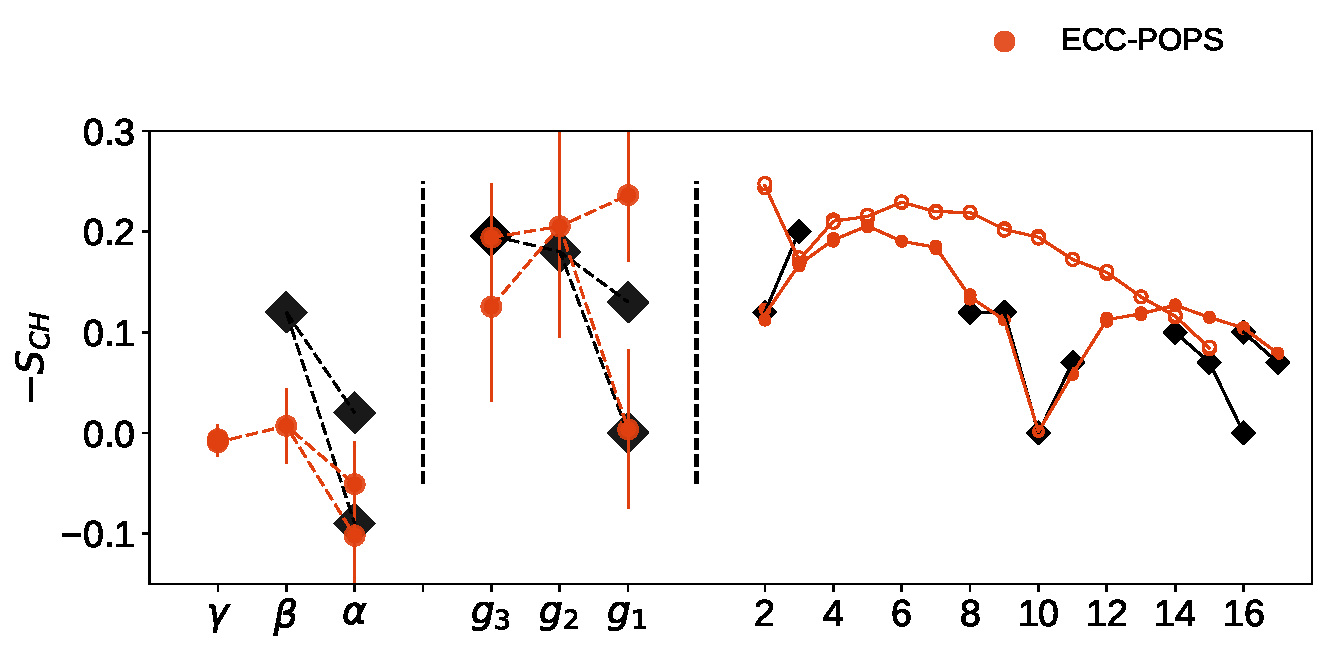
\includegraphics[width=\figwidth]{../Fig/order_parameters_actual_pure-POPS.pdf} \\
  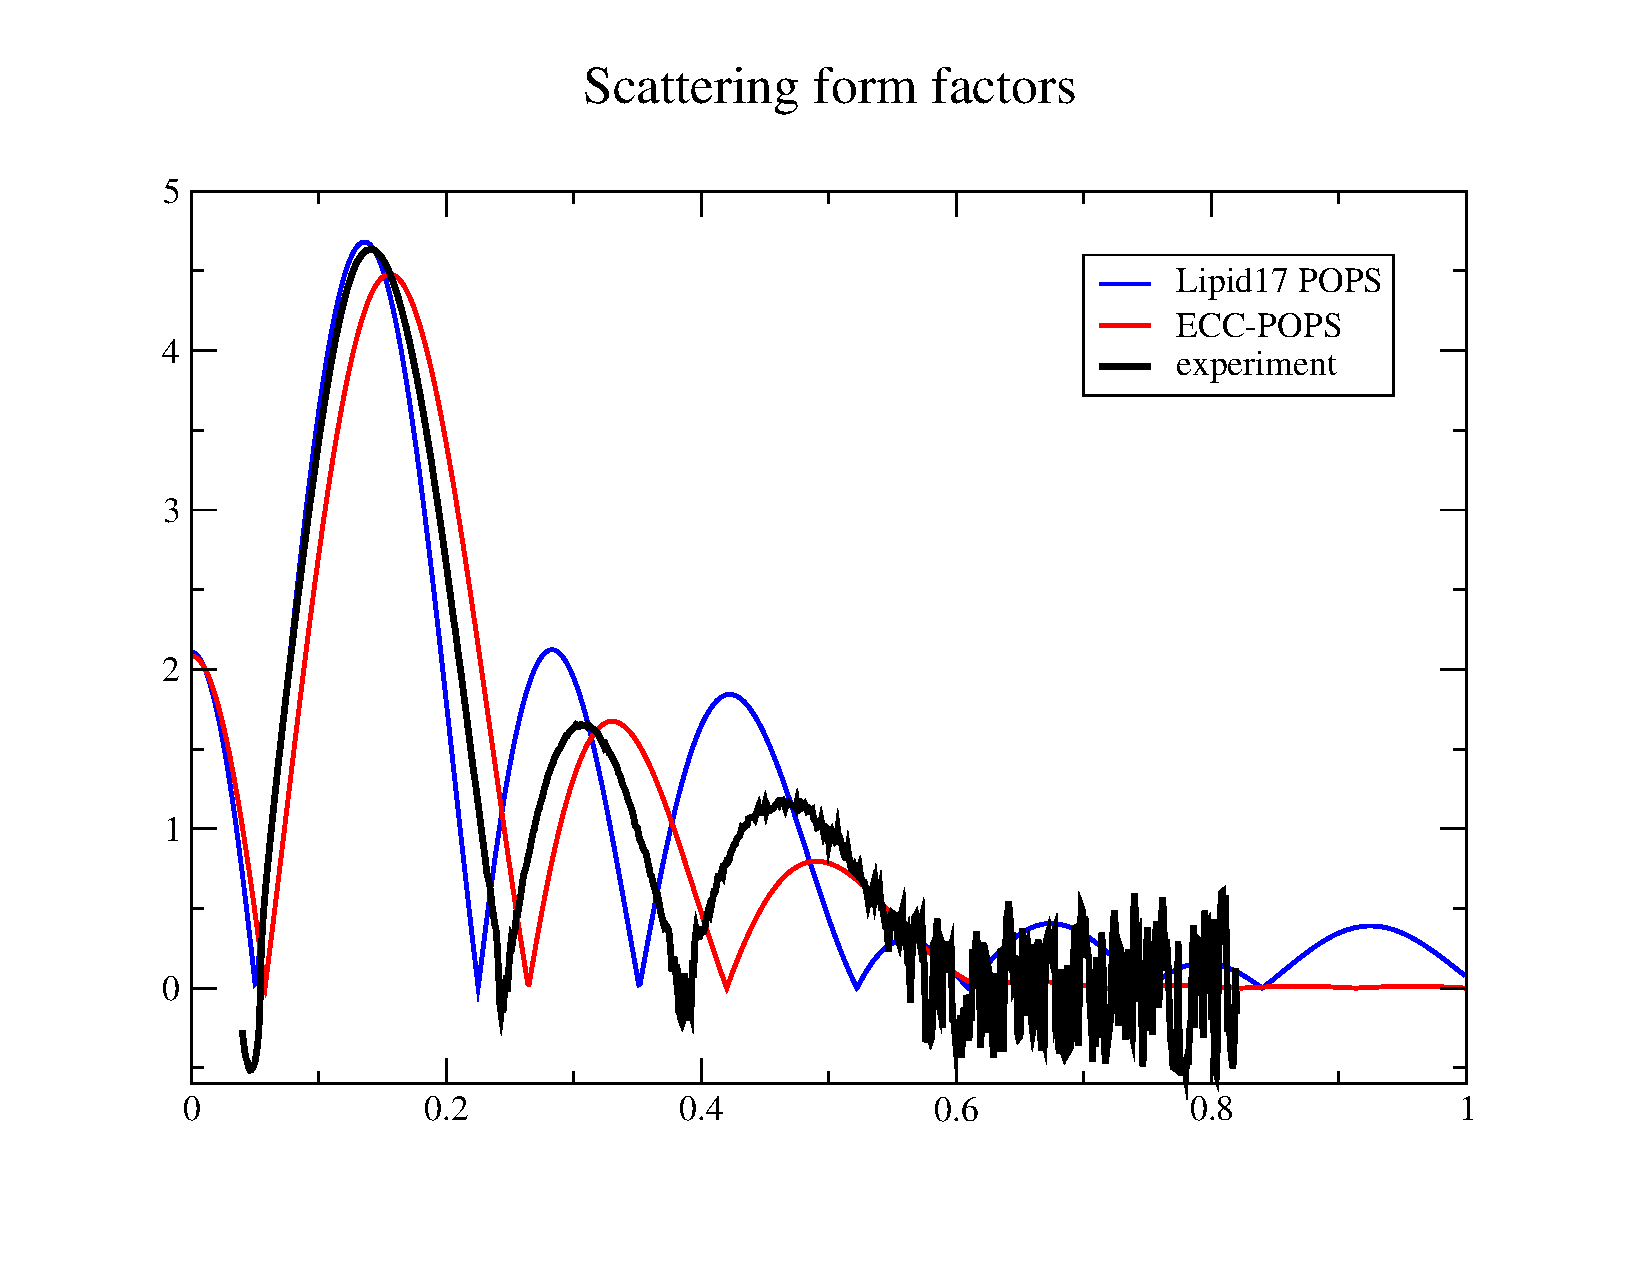
\includegraphics[width=0.7\figwidth]{../Fig/form-f_l17-ecc-pops-exp_compar.pdf} 
  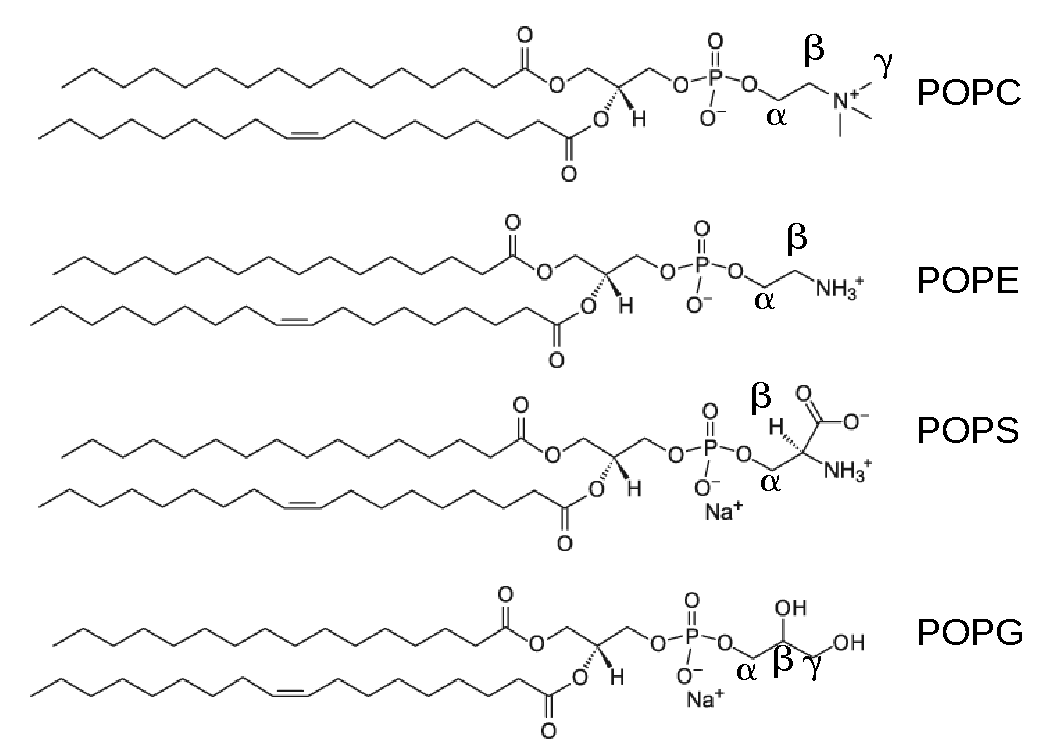
\includegraphics[width=0.55 \figwidth]{../Fig/lipids_chemfig.pdf} 
  \caption{\label{simVSexpNOions} 
    X-ray scattering form factors from simulations with the Lipid17 \cite{lipid17-future} and 
    the ECC-POPS models compared with experiments~\cite{SDP-CHARMM36_comparison_paper_Samuli-knows} at 298~K. 
    The disagreements between ECC-POPS model and experiment 
    may come from an intrinsincally incorrect structure of the head group (and, hence, electron density in the region), 
    however, lipid packing and overall membrane properties 
    may be still caputured well enough -- after considering areas per lipid reported in Table~\ref{tab:apls}.  \\
    Order parameters of POPS head group, glycerol backbone and acyl chains  
    from simulations with the Lipid17 \cite{lipid17-future} and the ECC-POPS models 
    compared with \emph{experiments at 300~K (check and change)}. 
    Open/closed symbols are used for palmitoyl/oleoyl chains of POPS. \\
    The chemical structure of POPS and the labeling of the carbon segments. 
  }  
\end{figure} 
 
\begin{table}[tb!] 
  \caption{Values of the area per lipid (APL) of POPS bilayers with only \ce{Na^+} counterions. \label{tab:apls} 
  } 
  \begin{tabular}{l|c c} 
    model          & APL (\AA$^2$)   & Temperature [K] \\ 
    \hline 
    Lipid14                   & 53.5$\pm$ 0.8  &  298 \\ 
    \hline 
    ECC-POPS                & 60.3$\pm$ 0.6  &  298       \\ 
    \hline 
    experiment \cite{SDP-CHARMM36_comparison_paper_Samuli-knows} & 62.3  &  298    \\ 
    \hline 
  \end{tabular} 
\end{table} 
 
 

 
 
\subsection{Electrometer concept in negatively charged membranes with various cations} 
 
Preliminary results are plotted in the figures in this section. 
Beware! -- the y-axis scales are variable!
Colours:
\begin{itemize}
  \item Red -- ECC-lipids, ECC-ions
  \item Blue -- Lipid14/17, Dang ions
\end{itemize}

Changes of the lipid bilayer head group order parameters extracted from simulations and 
experiments \cite{roux90} are shown in Figs.~\ref{fig:delta_ordPar_KCl}, \ref{fig:delta_ordPar_NaCl} 
and~\ref{fig:delta_ordPar_CaCl} as functions of KCl, NaCl or CaCl$_2$ concentrations,
and in Figs.~\ref{fig:delta_ordPar_NaCl_PC-PS_mix} as a function of PC and PS content. 



% ============================== 
% ==  ECC-lipids plots ========= 
% ==     and           ========= 
% ==  Lipid14/17 plots ========= 
% ============================== 
\begin{figure}[htb!] 
  \centering 
  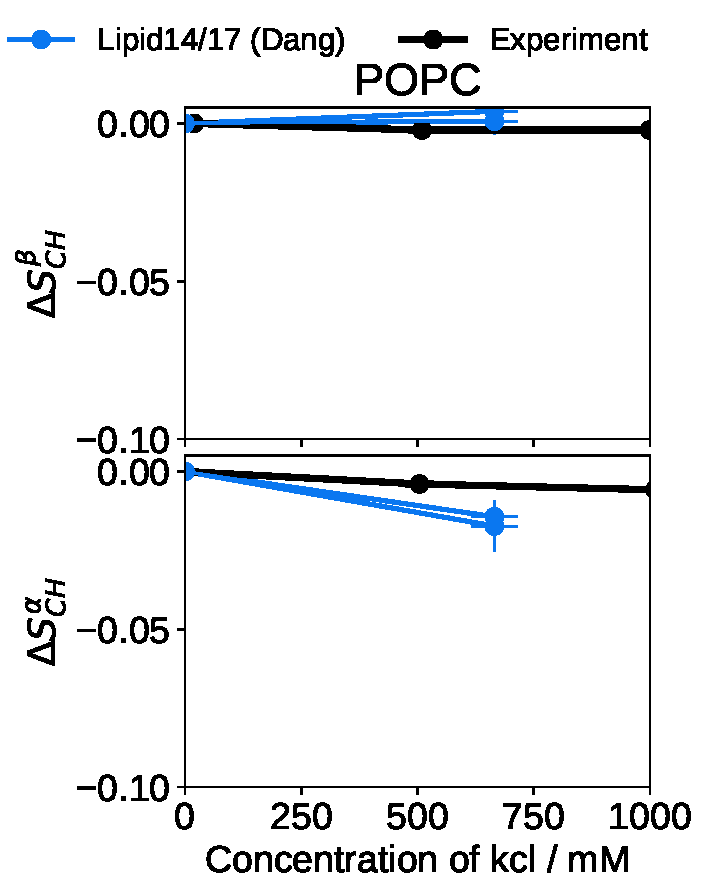
\includegraphics[width=\figwidth]{../Fig/l17/order_parameters_changes_A-B_POPC_kcl.pdf} 
  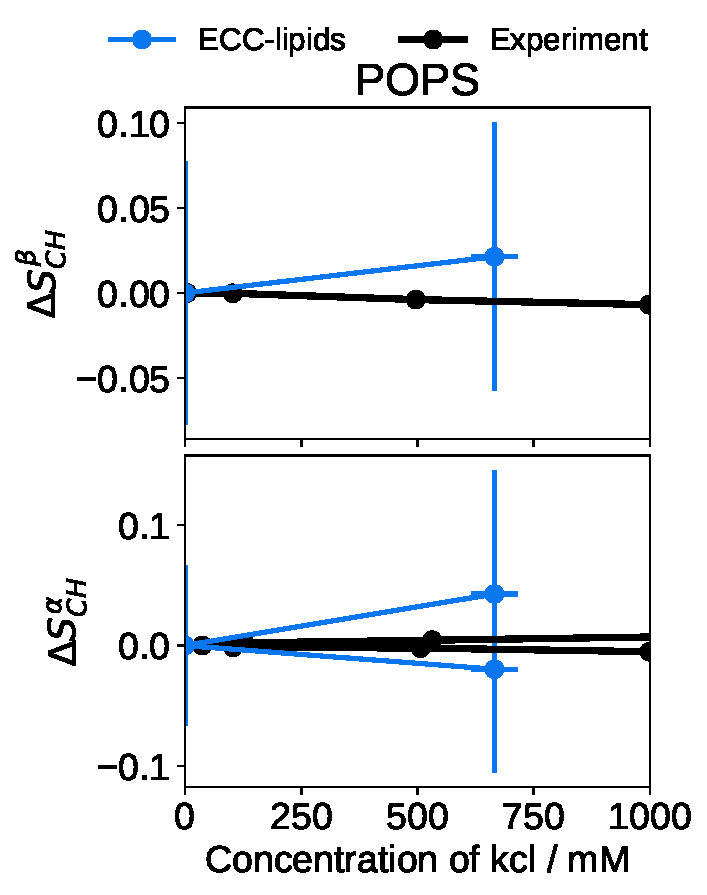
\includegraphics[width=\figwidth]{../Fig/l17/order_parameters_changes_A-B_POPS_kcl.pdf} 
  \caption{\label{fig:delta_ordPar_KCl_l17} 
    Changes of the head group order parameters of a POPC:POPS 5:1 bilayer as a function of KCl concentration 
    in bulk ($C_{ion}$) from simulations with different force fields at 298 K together with  
  } 
\end{figure} 
 
\begin{figure}[htb!] 
  \centering 
  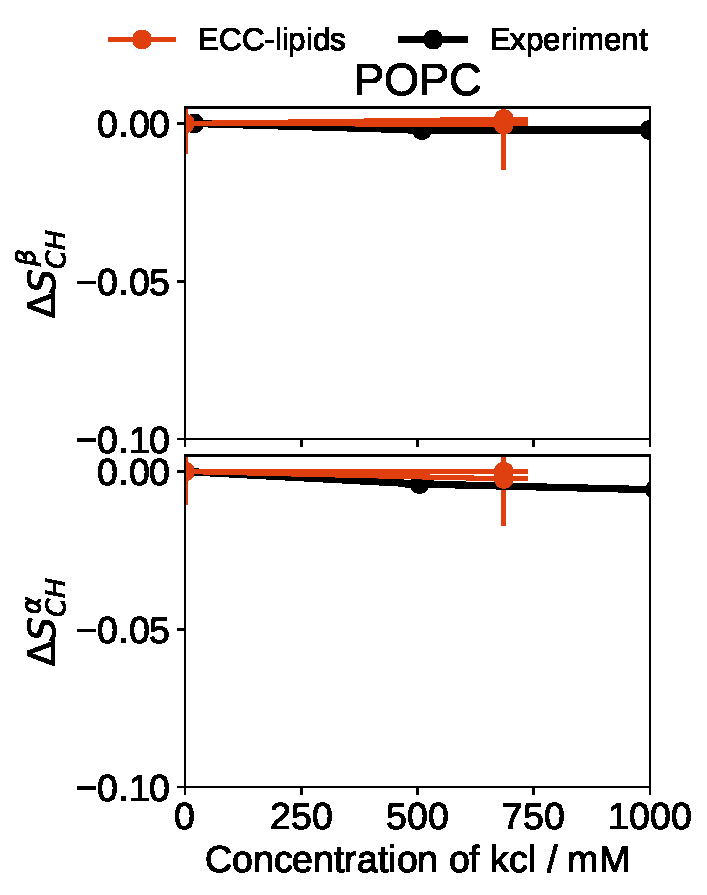
\includegraphics[width=\figwidth]{../Fig/order_parameters_changes_A-B_POPC_kcl.pdf} 
  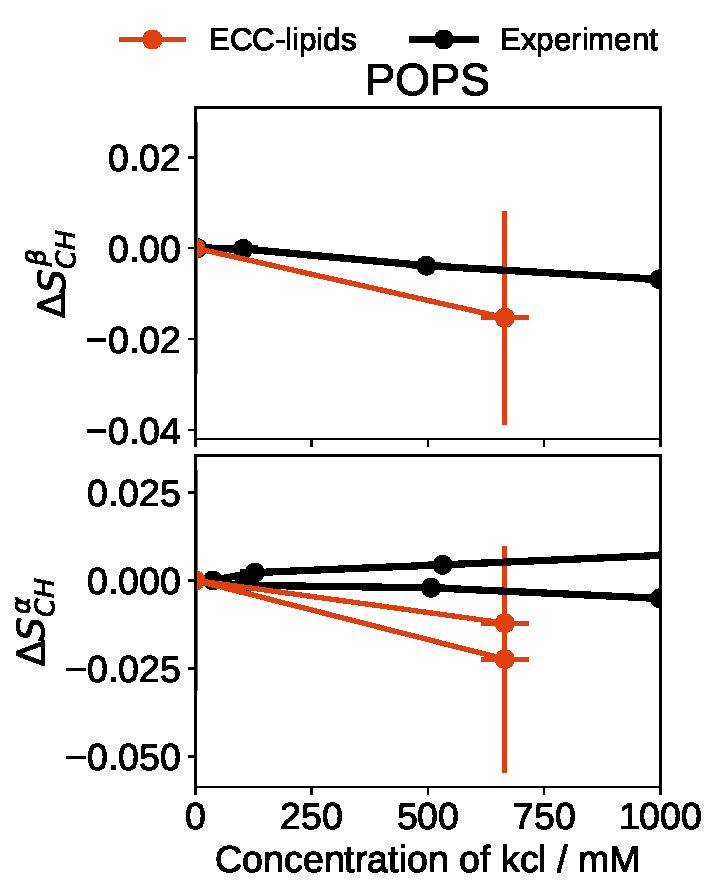
\includegraphics[width=\figwidth]{../Fig/order_parameters_changes_A-B_POPS_kcl.pdf} 
  \caption{\label{fig:delta_ordPar_KCl} 
    Changes of the head group order parameters of a POPC:POPS 5:1 bilayer as a function of KCl concentration 
    in bulk ($C_{ion}$) from simulations with different force fields at 298 K together with  
  } 
\end{figure} 
 
 
\begin{figure}[htb!] 
  \centering 
  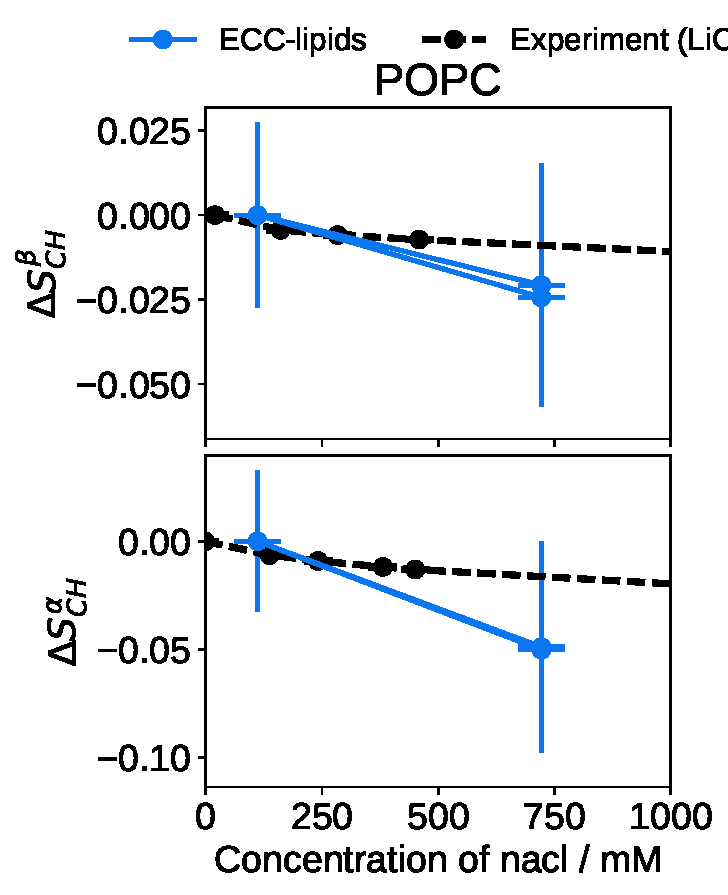
\includegraphics[width=\figwidth]{../Fig/l17/order_parameters_changes_A-B_POPC_nacl.pdf} 
  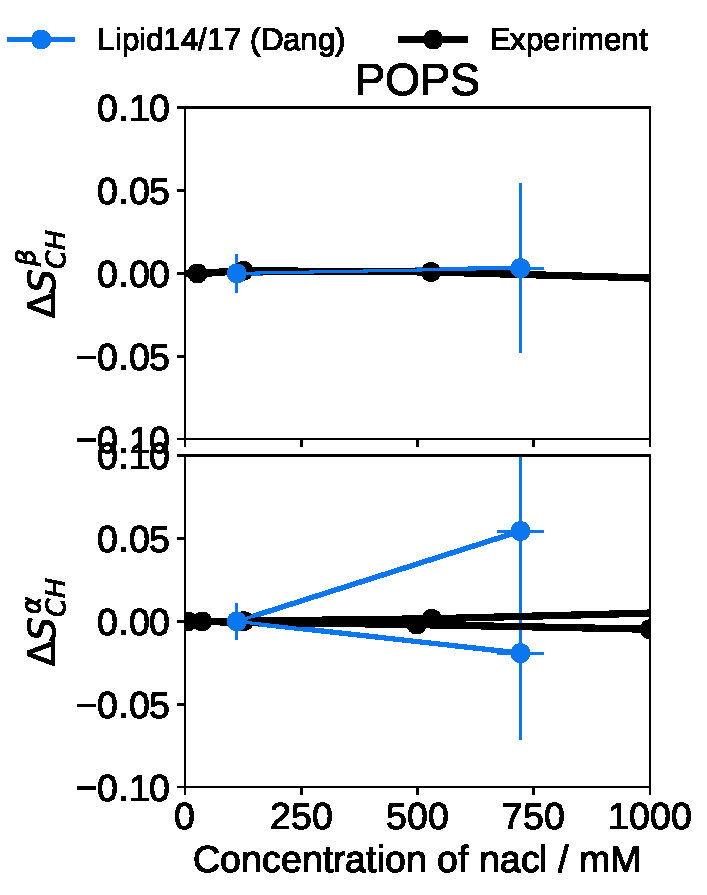
\includegraphics[width=\figwidth]{../Fig/l17/order_parameters_changes_A-B_POPS_nacl.pdf} 
  \caption{\label{fig:delta_ordPar_NaCl_l17} 
    Changes of the head group order parameters of a POPC:POPS 5:1 bilayer as a function of NaCl concentration 
    in bulk ($C_{ion}$) from simulations with different force fields at 298 K together with  
  } 
\end{figure} 

\begin{figure}[htb!] 
  \centering 
  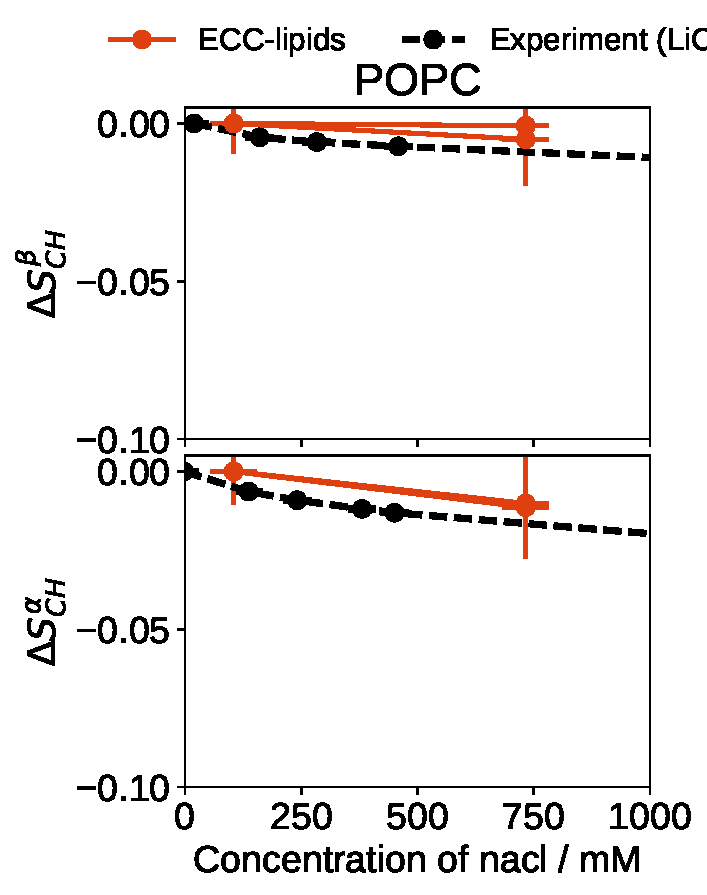
\includegraphics[width=\figwidth]{../Fig/order_parameters_changes_A-B_POPC_nacl.pdf} 
  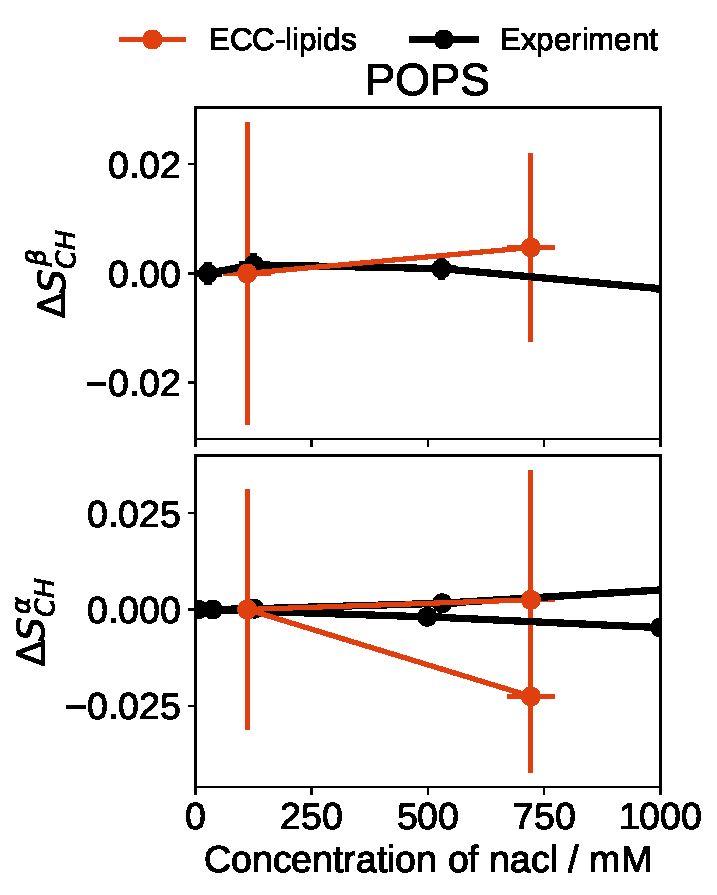
\includegraphics[width=\figwidth]{../Fig/order_parameters_changes_A-B_POPS_nacl.pdf} 
  \caption{\label{fig:delta_ordPar_NaCl} 
    Changes of the head group order parameters of a POPC:POPS 5:1 bilayer as a function of NaCl concentration 
    in bulk ($C_{ion}$) from simulations with different force fields at 298 K together with  
  } 
\end{figure} 
 

\begin{figure}[htb!] 
  \centering 
  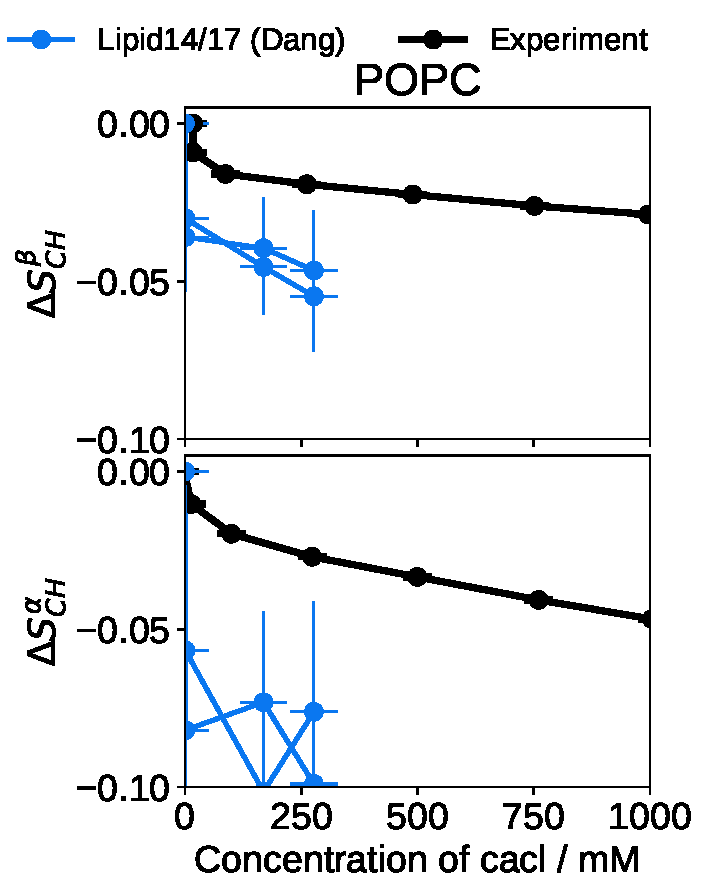
\includegraphics[width=\figwidth]{../Fig/l17/order_parameters_changes_A-B_POPC_cacl.pdf} 
  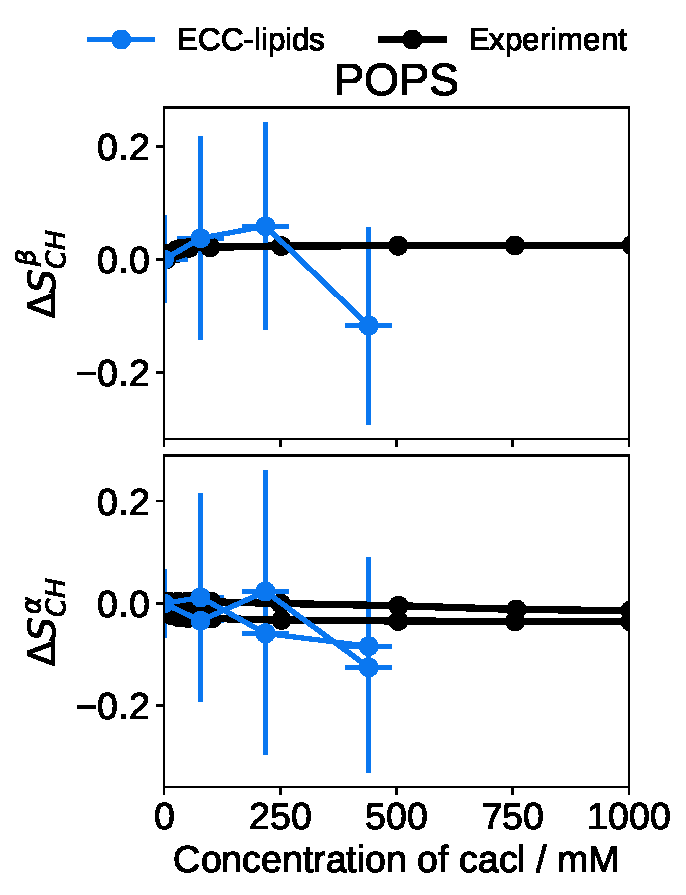
\includegraphics[width=\figwidth]{../Fig/l17/order_parameters_changes_A-B_POPS_cacl.pdf} 
  \caption{\label{fig:delta_ordPar_CaCl_l17} 
    Changes of the head group order parameters of a POPC:POPS 5:1 bilayer as a function of CaCl concentration 
    in bulk ($C_{ion}$) from simulations with different force fields at 298 K together with  
  } 
\end{figure} 
 
\begin{figure}[htb!] 
  \centering 
  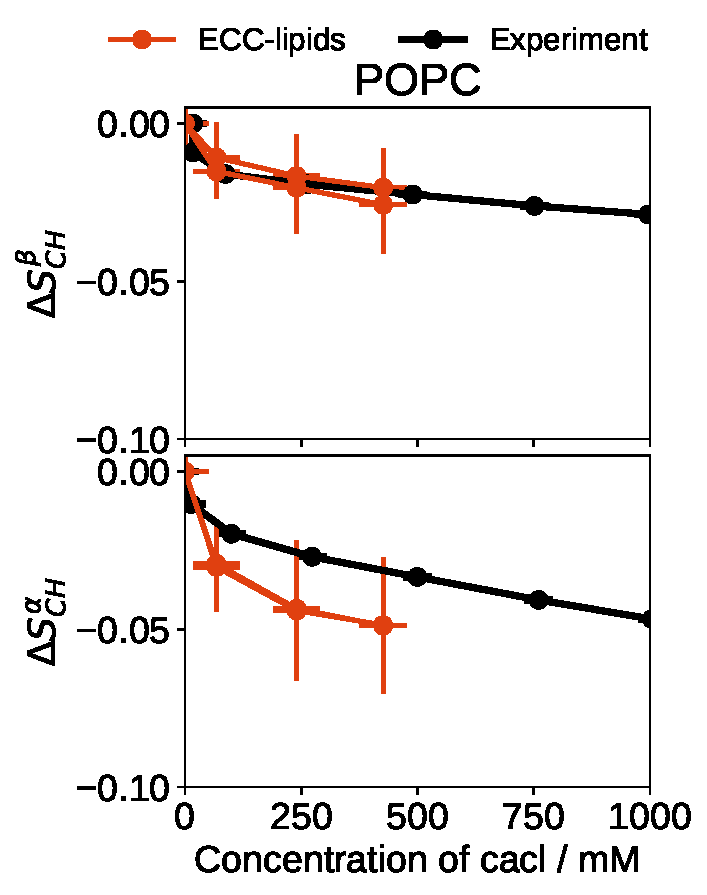
\includegraphics[width=\figwidth]{../Fig/order_parameters_changes_A-B_POPC_cacl.pdf} 
  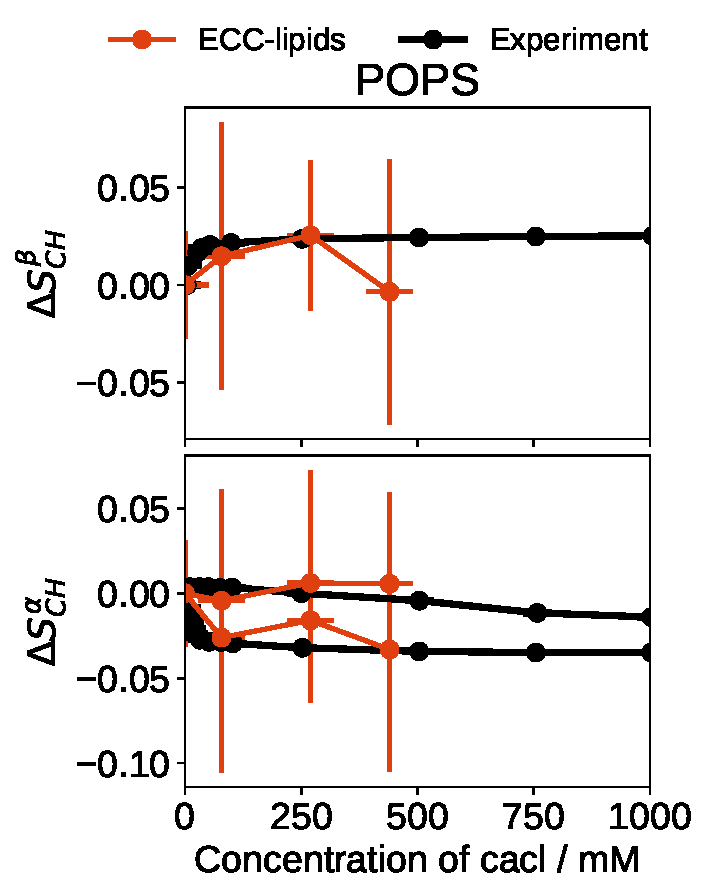
\includegraphics[width=\figwidth]{../Fig/order_parameters_changes_A-B_POPS_cacl.pdf} 
  \caption{\label{fig:delta_ordPar_CaCl} 
    Changes of the head group order parameters of a POPC:POPS 5:1 bilayer as a function of CaCl concentration 
    in bulk ($C_{ion}$) from simulations with different force fields at 298 K together with  
  } 
\end{figure} 



\begin{figure}[htb!] 
  \centering 
  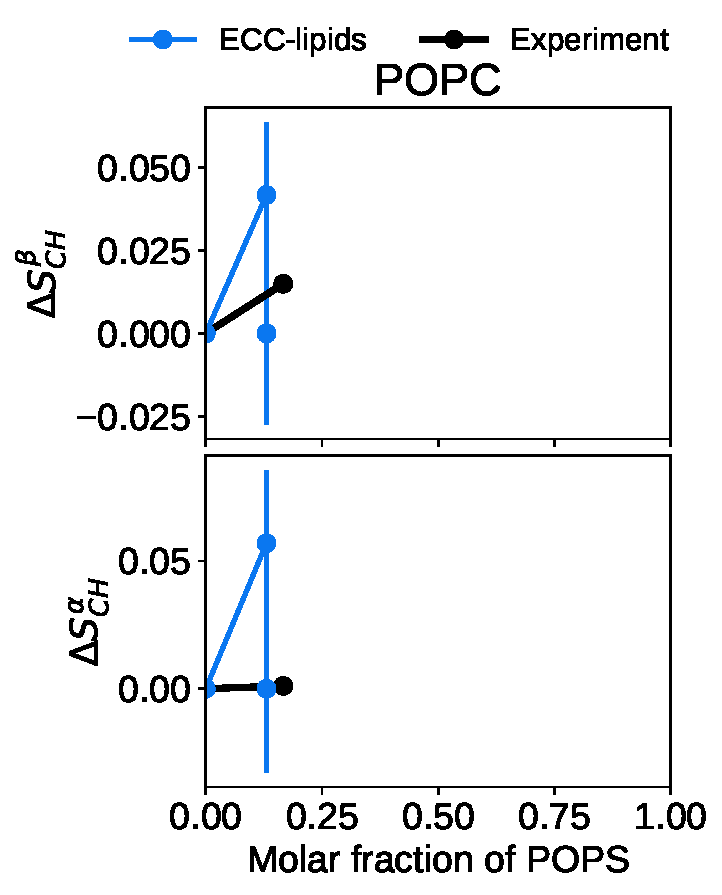
\includegraphics[width=\figwidth]{../Fig/l17/order_parameters_changes_A-B_PC-PS_mix_POPC_nacl.pdf} 
  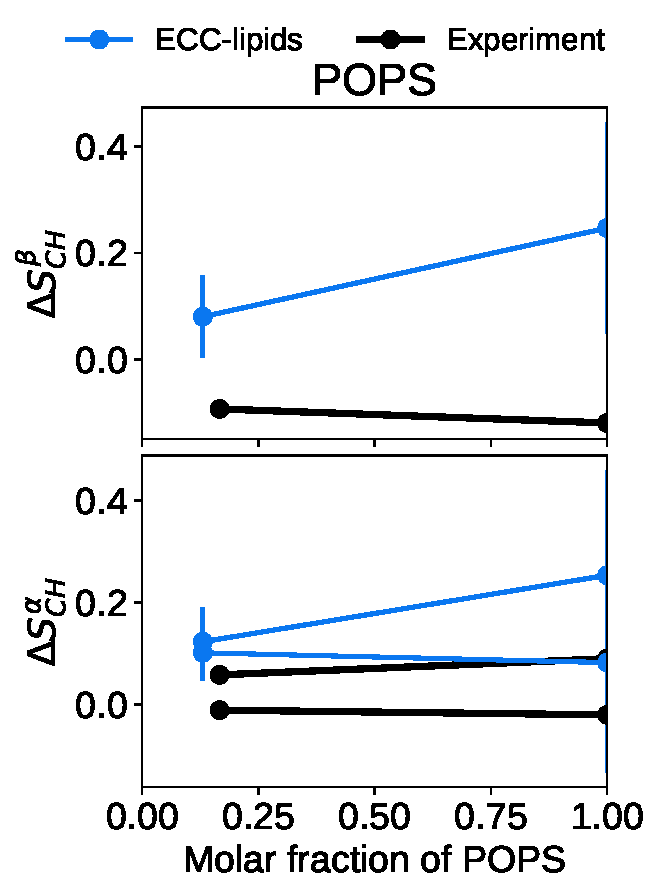
\includegraphics[width=\figwidth]{../Fig/l17/order_parameters_changes_A-B_PC-PS_mix_POPS_nacl.pdf} 
  \caption{\label{fig:delta_ordPar_NaCl_PC-PS_mix_l17} 
    Changes of the head group order parameters of a POPC:POPS 5:1 bilayer as a function of PS content.
    Experimental points have inherent systematic error, as they come from different experiments.
    A complete series of points can be found (?) in \cite{roux90} -- which is to be added to the plot.
  } 
\end{figure} 
 
\begin{figure}[htb!] 
  \centering 
  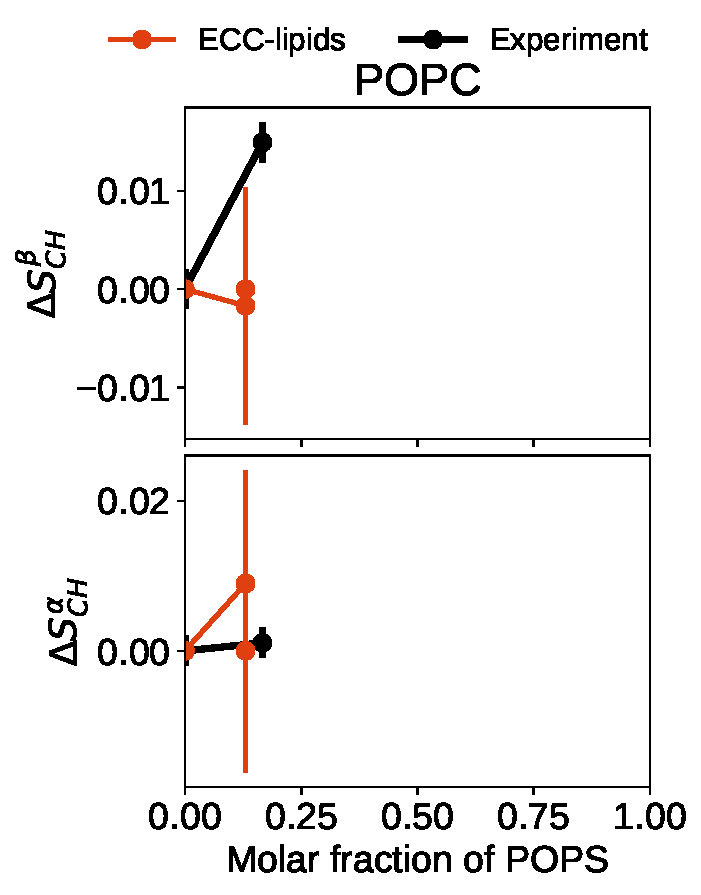
\includegraphics[width=\figwidth]{../Fig/order_parameters_changes_A-B_PC-PS_mix_POPC_nacl.pdf} 
  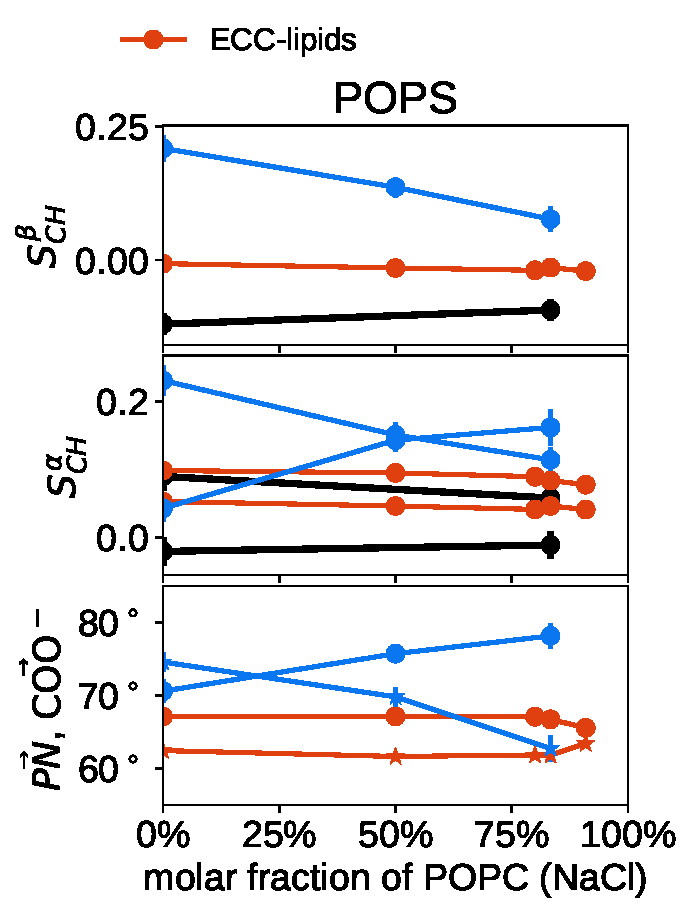
\includegraphics[width=\figwidth]{../Fig/order_parameters_changes_A-B_PC-PS_mix_POPS_nacl.pdf} 
  \caption{\label{fig:delta_ordPar_NaCl_PC-PS_mix} 
    Changes of the head group order parameters of a POPC:POPS 5:1 bilayer as a function of PS content
    Experimental points have inherent systematic error, as they come from different experiments.
    A complete series of points can be found (?) in \cite{roux90} -- which is to be added to the plot.
  } 
\end{figure} 



 
 
 


\subsection{Molecular interaction and binding affinities of K$^+$, Na$^+$ or Ca$^{2+}$  cations to the mixed POPC:POPS (5:1) membrane} 
\label{sec:affinity} 

Provide density plots and show, where and how the cations bind to the membrane. 

\textbf{Where do the cations bind?} 
The affinity towards PC and PS lipids and some of their groups was evaluated 
by counting contacts between the cation and the oxygen atoms of the lipids
similarly as was done in \cite{melcr18}. 
The threshold for counting a contact was set to be $0.3 \mathrm{nm}$, 
which encompasses the first peak of radial distribution function between the cations and the oxygen atoms of the lipids. 
In Table~\ref{tab:binding}, there are percentages of the membrane-bound calcium population for various membrane moieties. 
Although the lipid ratio in the membrane is 5~PC:1~PS,
half of the total population of calcium cations is bound to PS lipids
with 7\% bound only to them. 
This corroborates the intrinsincally higher affinity of PS lipids to calcium cations compared to PC lipids. 
The population analysis also suggests 
that the calcium cations prefer to reside in the phosphate region of the membrane. 
Hence, the carboxylate group in PS is coordinated to the cations bound in that region. 
The increased response of head group order parameters $\alpha$ and $\beta$ of PC 
in mixed 5~PC:1~PS bilayer compared to pure PC
is due to higer affinity of the membrane mediated by even a relatively small fraction (1/6) of PS lipids. 
This is in line with the steep onset of the response of the PS head group order parameters at lower concentrations.
The complex response of the head group order parameters of PS lipids 
is due to the confomational change of the carboxylate group that is attracted more towards the phosphate region. 
In order to examine whether the carboxylate and phosphate groups in PS are bound 
to the same calcium cation or rather different cations, 
more detailed analysis is required. 
\todo{Detailed analysis of the interactions of cations and PC/PS head groups using MSM.}


 
\begin{table}[tb!] 
  \caption{Bulk concentrations of Ca$^{2+}$ (C$_b$), 
           and the percentages of Ca$^{2+}$ bound to 
           either to PC or PS, 
           to PC or PS without phosphate group,
           to PC or PS without carboxylate group,
           to PC and PS at the same time,
           only to PC, 
           and only to PS 
           in a mixed POPC:POPS (5:1) bilayer. 
          \label{tab:binding}} 
  \begin{tabular}{l| c | c c c c c c } 
    model                  & $C_{ion}\,/\,\mathrm{mM}$ & PC+PS  &  PC+PS no PO$_4$ & PC+PS no COO$^-$ & PC-$Ca^{2+}$-PS  & PC & PS  \\ 
    \hline 
    ECC-lipids             &  $240\pm 10 $             & 100    &   98-99          & 100              & 43               & 50 &  7  \\
    \hline 
    Lipid14/17             &  $280\pm 10 $             & 100    &   ---            & ---              & ---              & ---& --- \\
    \hline 
    \todo{transpose this table and remove the comparison with Lipid14/17}
  \end{tabular} 
\end{table} 
 
 
%\begin{figure}[htbp!] 
%  \centering 
%  \includegraphics[height=19.9cm]{../Fig/}
%  \caption{\label{fig:cacl-dens} 
%    Number density profiles of \ce{Ca^{2+}}, \ce{Na^{+}} and \ce{Cl^-} along membrane normal axis 
%    for different force fields. 
%    } 
%\end{figure} 
 
%\subsection{Molecular interactions between K$^+$, Na$^+$ or Ca$^{2+}$ cations and mixed POPC:POPS membrane} 
 
%\subsection{Binding stoichiometry of cations to mixed POPC:POPS membrane} 

%\subsection{Residence times of cations in the mixed POPC:POPS membrane} 
 
%\begin{figure}[tb!] 
%  \centering 
%  \includegraphics[width=8.0cm]{../Fig/ipython_nb/stoichiometry_NaCl-CaCl2_comparison_Ecc-lipids.pdf} \\ 
%  \caption{\label{fig:cacl_complexes} 
%      Relative probabilities of existence of \ce{Na^{+}} or \ce{Ca^{2+}} complexes 
%      with a certain number of POPS lipids.  
%      \ce{Na^{+}} complexes were evaluated from the simulation with 1~M concentration; 
%      and \ce{Ca^{2+}} complexes were evaluated from the simulation with 287~mM concentration. 
%  } 
%\end{figure} 
 
 

\subsection{Electronic Continuum Correction as a generally applicable model polarizability?}

Show the successes and possible \emph{limits} of ECC applied on top of various models \cite{melcr18, martinek17, Pluharova2014, kohagen14, kohagen16}. 

After validation above, it can be an option to show results also for systems, for which we have no experiments. 

 
 
 
 
 
\section{Conclusions} 

 
 
 
% If you have acknowledgments, this puts in the proper section head. 
\begin{acknowledgement} 
% Put your acknowledgments here. 
P.J. acknowledges support from the Czech Science Foundation (grant no. 16-01074S)  
and from the Academy of Finland via the FiDiPro award. 
Computational resources were supplied by the Ministry of Education, Youth and Sports 
of the Czech Republic under the Projects CESNET (Project No. LM2015042) and CERIT-Scientific 
Cloud (Project No. LM2015085) provided within the program Projects of Large Research, 
Development and Innovations Infrastructures. 
O.H.S.O. acknowledges financial support from 
Integrated Structural Biology Research Infrastructure of 
Helsinki Institute of Life Science (Instruct-HiLIFE). 
\end{acknowledgement} 
 
\begin{suppinfo} 
 
%A listing of the contents of each file supplied as Supporting Information 
%should be included. For instructions on what should be included in the 
%Supporting Information as well as how to prepare this material for 
%publications, refer to the journal's Instructions for Authors. 
 
%The following files are available free of charge. 
%\begin{itemize} 
%  \item Filename: brief description 
%\end{itemize} 
 
\end{suppinfo} 
 
 
\bibliography{refs.bib} 
 
\end{document} 
 

